\iffalse

INSTRUCTIONS:

  Clip out the ********* INSERT HERE ********* bits below and insert
appropriate TeX code.  Once you are done with your file, run

  ``latex sample.tex''

from the Athena shell.  If your TeX code is clean, the latex will exit
back to a prompt.  Once this is done, run

  ``dvips -t letter -f sample.dvi > sample.ps''

You can then convert the PostScript output to PDF:
  ``ps2pdf sample.ps''

\fi
\documentclass[11pt]{article}
\usepackage{amsfonts}
\usepackage{latexsym}
\usepackage{amsmath}
\usepackage{amsfonts,amssymb,amsthm,epsfig,epstopdf,titling,url,array}
\setlength{\oddsidemargin}{.25in}
\setlength{\evensidemargin}{.25in}
\setlength{\textwidth}{6in}
\setlength{\topmargin}{-0.4in}
\setlength{\textheight}{8.5in}


\newcommand{\handout}[5]{
   \renewcommand{\thepage}{#1-\arabic{page}}
   \noindent
   \begin{center}
   \framebox{
      \vbox{
    \hbox to 5.78in { {\bf 6.867: Machine Learning} \hfill Due: Sep 30th }
       \vspace{4mm}
       \hbox to 5.78in { {\Large \hfill #1: #5  \hfill} }
       
       
      }
   }
   \end{center}
   \vspace*{4mm}
}

\newcommand{\al}{\alpha}
\newcommand{\Z}{\mathbb Z}

\begin{document}

\handout{Homework 1}{Due Date here}{Instructor Here}
{Your T.A. Here}{Yunming Zhang}


\section{Problem 1 Implement Gradient Descent}

\subsection{Algorithm}
The optimization goal is to minimize function $y = \bf{F(X)}$. We update the independent variable $\bf{X}$ with the gradient of function $\bf{F(X)}$ and stepsize $\gamma$.

\begin{equation}
\bf{X_{n+1}} = \bf{X_{n}} - \gamma \cdot \bigtriangledown F(X_{n})
\end{equation}
\\
We stop the iteration when it converges, i.e., the difference between two consecutive values of the function is smaller than the convergence criteria $\delta$.

\begin{equation}
|y_{n+1} - y_n| < \delta
\end{equation}
\\
Two functions are used to evaluate the algorithm:

\begin{figure}[h]
 \centering
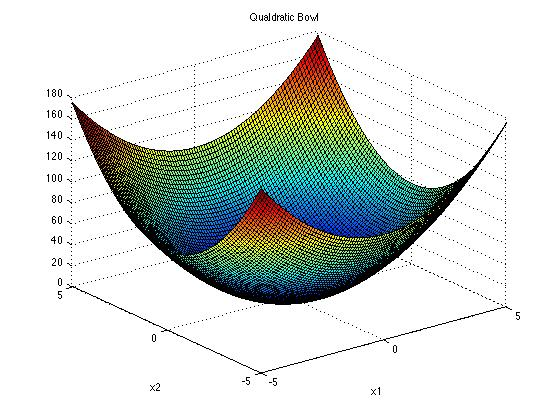
\includegraphics[height=2.2in]{figures/p1_QualdraticBowl} 
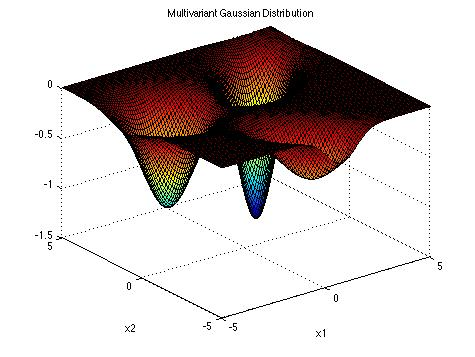
\includegraphics[height=2.2in]{figures/p1_MultivariantGaussian} 
    \caption{Plots of two functions}
    \label{fig:functions}
\end{figure}

A qualdratic bowl function, which is convex:
\begin{equation}
F_1(X) = 3 {x_1}^2+4 {x_2}^2
\end{equation}

A superposition of three psedo-multivariate gaussian distributions (they are scaled but not real multivariate gaussian distributions), which is non-convex with three local minimals:
\begin{equation}
F_2(X) = \sum_{i=1}^3 a_i \cdot e^{-\frac{1}{2} (X - \mu_i)^T \Sigma_i ^{-1} (X - \mu_i)}
\end{equation}
where 
\[
a_1 = 1.5, a_2 = 1, a_3 = 0.5
\]
\[
\mu_1 = [2, 2]^T, \mu_2 = [-3,1]^T, \mu_3 = [0,-4]^T,\]
\[
\Sigma_1 =\left( \begin{array}{ccc}
1 & 0.5 \\
0.5 & 1  \end{array} \right),
\Sigma_2 =\left( \begin{array}{ccc}
1 & 0 \\
0 & 1  \end{array} \right),
\Sigma_3 =\left( \begin{array}{ccc}
1 & -0.7 \\
-0.7 & 1  \end{array} \right)
\]




\subsection{Initial Guess, Step Size, and Convergence Criteria}

For $F_1$, no matter where the initial guess is, with appropriate step size and convergence criteria, the algorithm will converge at last. Differerent initial guesses result in different iteration numbers needed to converge. The further the initial guess is from the real optimal, the more iterations it is needed to converge. The left plot of Figure~\ref{fig:Itr} shows that, different inital points result in differernt trajectory of converge. The three initial points are $[10,0], [0,10], [7.07,7.07]$ respectively. The right plot of Figure~\ref{fig:Itr} shows that, the number of iteration increases as the distance from the initial point to the real optimum increases. The Initial distance from the optimum varies from 0.01 to 10000, and the iteration number varies from 3 to 18. Here, step size is fixed to 0.1 and convergence threshold is 0.0001.

\begin{figure}[h]
 \centering
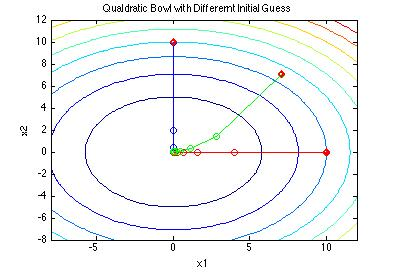
\includegraphics[height=2in]{figures/p1_QualdraticBowlWDifferenrtInitial} 
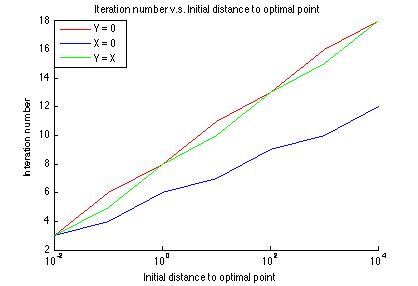
\includegraphics[height=2in]{figures/p1_QualdraticItrInit} 
    \caption{(Left) Iteration trajectory from different initial guess (Right) Iteration number v.s. Initial distance from the optimal}
    \label{fig:Itr}
\end{figure}

Next, we adjust the stepsize with the inital point and convergence threshold fixed (inital guess is [10,10], convergence threshold is 0.0001). The results in table~\ref{tab:ItrStep} show that, when the stepsize is relatively small, the iteration number decreases as the stepsize increases. However, after the stepsize is large enough, increase the stepsize will help reduce the number iteration no more. Here, when stepsize is 0.2, it takes longer to converge than stepsize is 0.1. If the stepsize further increase, the algorithm may not converge (when stepsize equal or larger than 0.3). From figure~\ref{fig:ItrStep} we can see that, when stepsize is big, the gradient descent trajectory can oscillate around the optimum. If it is too big, the oscillation can be unstable thus never converge.

Another observation is, a moderate stepsize (in this case 0.1) finds the minimum point of the function with the most accuracy. Thus it is crucial to choose an appropriate stepsize, not too big and not too small.

\begin{table}[h]
\centering
\caption{Number of Iteration \& Minimum found v.s. Stepsize} \label{tab:ItrStep} 
\begin{tabular}{ | c | c | c | c | c | c | c | c |  }
\hline 
Stepsize & 0.0001 & 0.0005 & 0.01 & 0.05 & 0.1 & 0.2 & 0.3 \\
\hline 
Iteration num & 878 & 201 & 106 & 22 & 11 & 17 & Not converge \\
\hline
Minimum found $y$ & 0.0081 & 0.0016 & 6.92e-4&9.38e-5 & 3.30e-6 & 3.18e-5\\
\hline
\end{tabular}
\end{table}

\begin{figure}[h]
 \centering
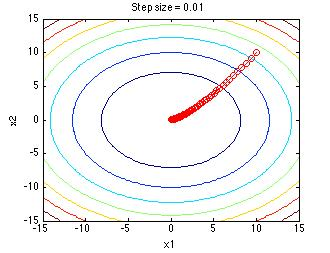
\includegraphics[height=2in]{figures/p1_QualStepSmall} 
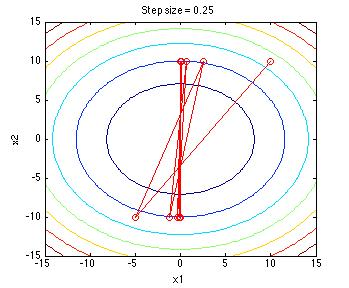
\includegraphics[height=2in]{figures/p1_QualStepBig} 
    \caption{Iteration trajectory with different stepsize (Left) Stepsize=0.01, (Right) Stepsize=0.25}
    \label{fig:ItrStep}
\end{figure}

Finally, we adjust the convergence criteria with the other attributes fixed (Inital guess = [10,10], stepsize = 0.1). Table~\ref{tab:ItrConve} shows that, the smaller the convergence criteria is, the more accurate the found minimum point is, however the longer it is to converge.
\begin{table}[h]
\centering
\caption{Number of Iteration \& Minimum found v.s. Convergence criteria} \label{tab:ItrConve} 
\begin{tabular}{ | c | c | c | c | c | c | c |  }
\hline 
Convergence Criteria & 0.00001 & 0.0001 & 0.001 & 0.01 & 0.1 & 1 \\
\hline 
Iteration num & 12 & 11 & 9 & 8 & 7 & 6  \\
\hline
Minimum found $y$ & 5.28e-7 & 3.30e-6 & 1.29e-4 & 8.05e-6 & 5.00e-3 & 3.15e-2\\
\hline
\end{tabular}
\end{table}


For $F_2$, the superpostion of multivariate gaussian distribution, most of the observations above still hold. The most different feature is summarized below.

In this case, the intial guess plays a more important role. Since the function is nonconvex and three local minimum exist, the minimum point found by the algorithm could be local minimal but not global minimal. In this case, $X = [2,2]$ is the global minimum. However starting from differerent point, the other local minimal points $X = [-3,1]$ and $X = [0,-4]$ may also be found (See Figure~\ref{fig:GaussianInit}). The gradient descent algorithm cannot avoid being trapped by the local minimums. Also, there are 'flat' area exists in this case. E.g. if we start from $X = [4,-4]$, the algorithm converge in two iterations without decsending to the optimums. A very small converge criteria is needed to avoid this. However the tradeoff between converge criteria and number of iteration should also be considered.

\begin{figure}[h]
\centering
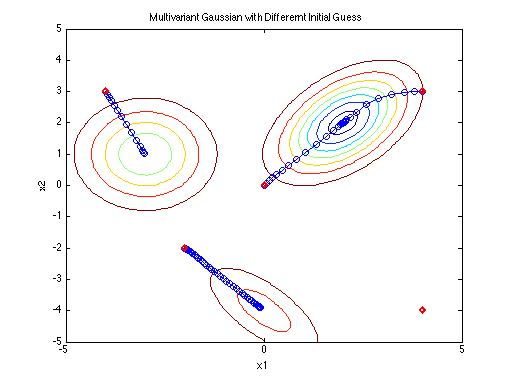
\includegraphics[height=3in]{figures/p1_MultivarianGaussianWDifferenrtInitial} 
    \caption{Iteration trajectory from different initial guess of the non-convex function}
    \label{fig:GaussianInit}
\end{figure}

To summarize, for gradient descent algorithm, it is important to choose an appropriate starting point to make sure it converge to global minimum instead of local minimum, as well as avoid being trapped on 'flat' area of a function. 
Stepsize needed to chosen carefully to make sure the algorithm converges, as well as converges fast enough.
Convergence criteria directly relates to the accuracy of the minimum point founds. Also it influence the speed of convergence.





\subsection{Analytical Gradient and Numerical Gradient }

The analytical gradient of the qualdratic bowl function $F_1(X)$ is:

\begin{equation}
\frac{\partial F_1(X)}{\partial x_1} = 6 x_1\\
\frac{\partial F_2(X)}{\partial x_2} = 8 x_1\\
\end{equation}\\
The analytical gradient of the function $F_2(X)$ is:

\begin{equation}
\bigtriangledown F_2(X) = \sum_{i=1}^3 a_i \cdot (-\Sigma_i ^{-1} (X - \mu_i)) e^{-\frac{1}{2} (X - \mu_i)^T \Sigma_i ^{-1} (X - \mu_i)}
\end{equation}\\
The numerical gradient we applied is:

\begin{equation}
\frac{\partial F(X)}{\partial x_i} = \frac{F(x_j,(x_i+\delta x)) - F(x_j,(x_i-\delta x))} {2 \delta x} \hspace{10 mm}  j\neq i
\end{equation}\\


For the qualdratic bowl function $F_1(X)$, we compare the analytical and numerical results on $9 \times 9$ points, given both $x_1$  and $x_2$ vary on 9 values: $[-1000 -100 -10 -1\  0\  1\  10\  100\   1000]$.
The difference between the two gradient are showed in Figure~\ref{fig:gradientCompare}.

\begin{figure}[h]

Difference between $\frac{\partial F(X)}{\partial x_1} $: \\
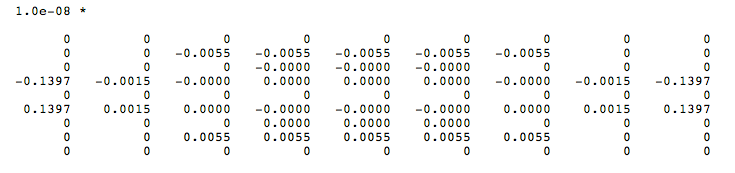
\includegraphics[height=1.5in]{figures/p13_compare1} 
Difference between $\frac{\partial F(X)}{\partial x_2} $: \\
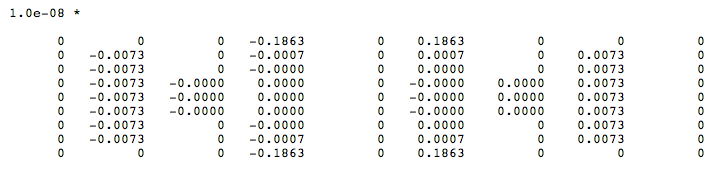
\includegraphics[height=1.5in]{figures/p13_compare2} 
    \caption{Screenshot of difference between the numerical and analytical gradient. }
    \label{fig:gradientCompare}
\end{figure}

Here $\delta = 0.1$. The difference between two gradients are controlled under the order of $10^{-8}$. Smaller $\delta$ will give even smaller difference between the analytical and numerical results.

$F_2(X)$ requires smaller $\delta$ to make sure the numerical gradient doesn't differ too much from the analytical one. With $\delta = 0.0001$, the difference between the two gradient can again be controlled under the order of $10^{-8}$.



\subsection{Compare Gradient Descent with $fminunc()$}





























\section*{Problem 2}

this is a separate tex file
You can also do more complex math formulas:
\[\Theta(n^2) = \sum_{i=0}^n i\]

\section{Problem 3}

\subsection{Part1}

{\bfseries Algorithm} \\
We first create a centered x data matrix Z. And then we cerate a centered y values.

\begin{equation}
z^{(i)}_{j} = x^{(i)}_{j} - \bar{x}_{j} \hspace{10 mm} 
y^{(i)}_{c} = y^{(i)} - \bar{y} \\
\end{equation}

Then we use the formula for calculating the error. It uses a $\lambda$ for regularizing the
weight terms. 

\begin{equation}
  E(w)= (Y_{c} - ZW)^T(Y_{c}-ZW) + \lambda W^TW \\
\end{equation}

We used a regularized term to calculate optimal weight using the following equation

\begin{equation}
  W_{ridge} = (Z^{T}Z + \lambda I)^{-1}Z^{T}Y_{c}
\end{equation}

{\bfseries Experimentation} \\
We have conducted a series of experimentation with the simple data from Bishop's Figure 1.4

%TODO: generate graphs to show the impact of increasing M (overfitting), but this is shown in the previou squestion
As M increases, the curve is more likely to overfit the data. 

We have conducted a series of experiments using M =1, M = 3 and M = 9 with varying lambdas. 


\begin{figure}[!htb]
\minipage{0.5\textwidth}
  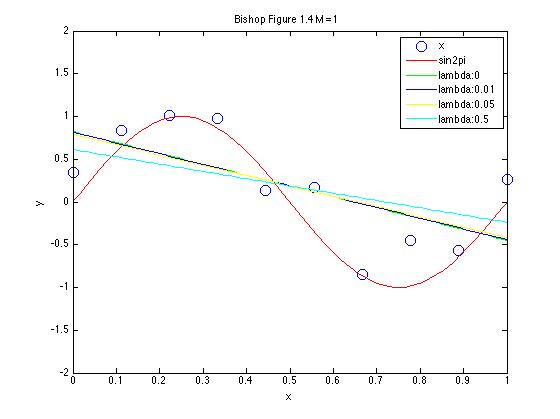
\includegraphics[width=\linewidth]{figures/p3_bishop_m=1}
  \caption{M = 1 with various lambdas}\label{fig:figures/p3_bishop_m=1}
\endminipage\hfill
\minipage{0.5\textwidth}
  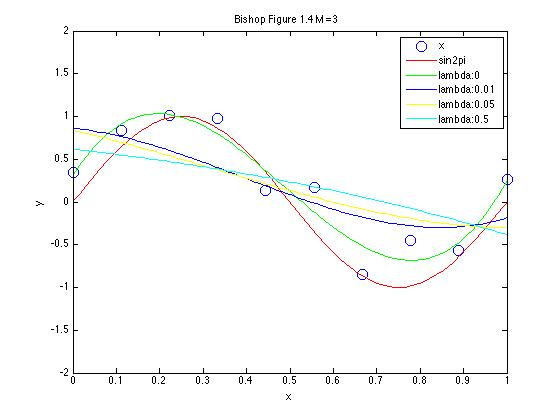
\includegraphics[width=\linewidth]{figures/p3_bishop_m=3}
  \caption{M = 3 with various lambdas}\label{fig:figures/p3_bishop_m=3}
\endminipage\hfill
\minipage{0.5\textwidth}%
  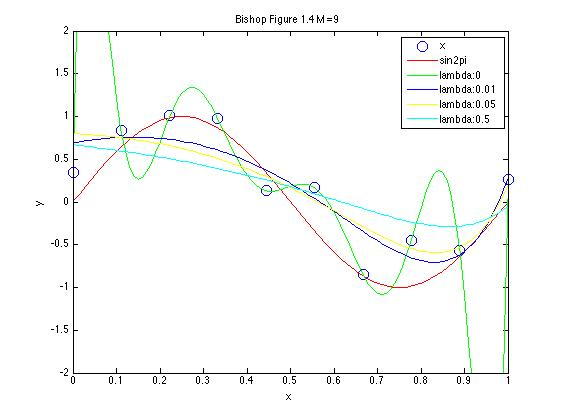
\includegraphics[width=\linewidth]{figures/p3_bishop_m=9}
  \caption{M = 9 with various lambdas}\label{fig:figures/p3_bishop_m=9}
\endminipage
\end{figure}



%% \begin{figure}[h]

%%   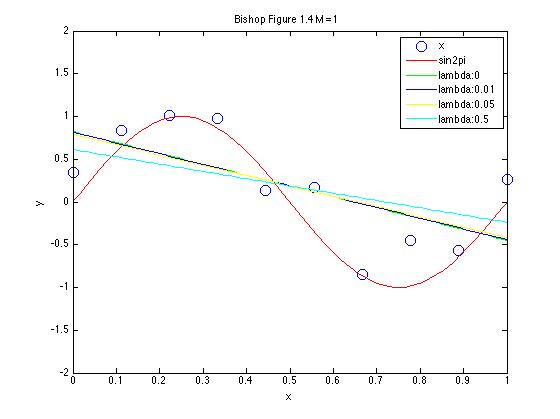
\includegraphics[width=0.5\textwidth]{figures/p3_bishop_m=1}
%%   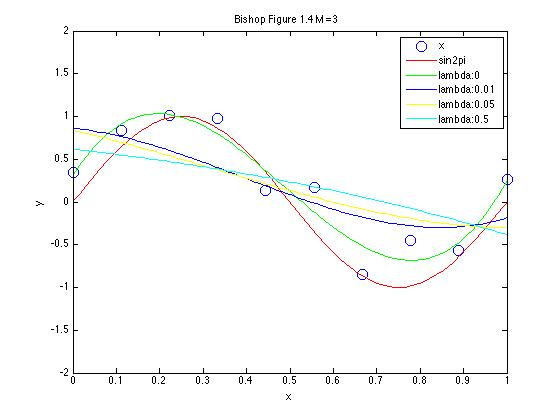
\includegraphics[width=0.5\textwidth]{figures/p3_bishop_m=3}
%%   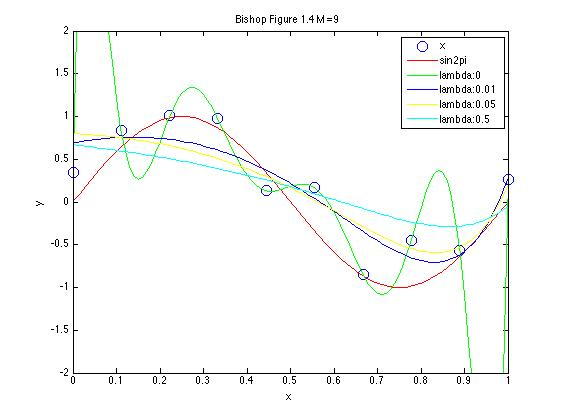
\includegraphics[width=0.5\textwidth]{figures/p3_bishop_m=9}

%% \end{figure}

we can see that for a smaller M, changing the lambda doesn't impact the performance as much. It bends the graph in the more general direction. For a large M, the lambda greatly reduces the overfitting problem. As a result, even with a large M, the model can be more generalized. 

\subsection{Part2}


%TODO: generate graphs to show the impact of increasing M (overfitting)

%TODO: generate graphs to show the inmpact of increaing lambda

%TODO: show that the models trained from data A is a lot better than model B


\subsection{Part3}

\section{Problem 4}

{\bfseries 4.1 Part1}

\begin{figure}[!htb]
\minipage{0.25\textwidth}
  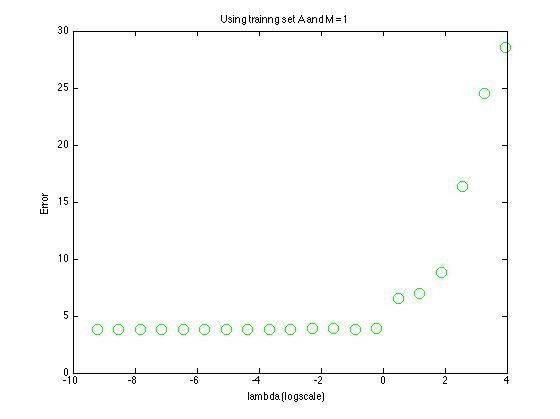
\includegraphics[width=\linewidth]{figures/p4_LAD_regressA_m=1}
\endminipage\hfill
\minipage{0.25\textwidth}
  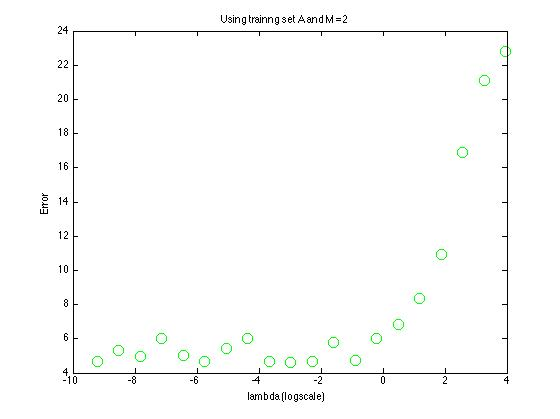
\includegraphics[width=\linewidth]{figures/p4_LAD_regressA_m=2}
\endminipage\hfill
\minipage{0.25\textwidth}                                                                                 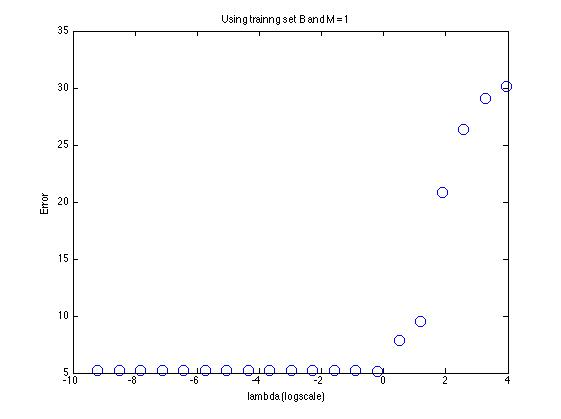
\includegraphics[width=\linewidth]{figures/p4_LAD_regressB_m=1}
\endminipage\hfill
\minipage{0.25\textwidth}
  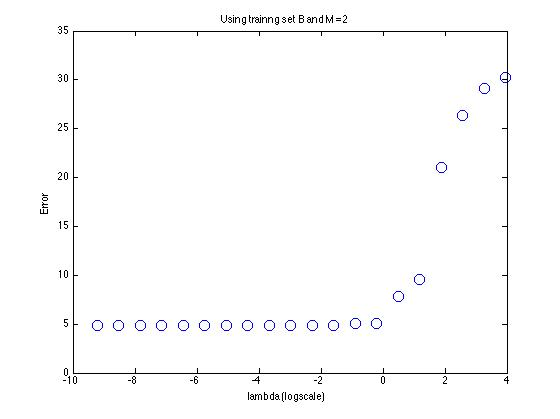
\includegraphics[width=\linewidth]{figures/p4_LAD_regressB_m=2}
\endminipage\hfill
\caption{LAD for set A,B and M = 1,2}\label{p4_LAD}
\end{figure}

Again we splitted the validation set into a validation and test set. Figure~\ref{p4_LAD} shows the result for M = 1,2 for LAD. My experiments on validation set shows that M = 1, M = 2 generates the
best results using both A and B. We carried out a series of experiments with varying values
of lambda, setting M = 2 and 3. I tested a few configurations with M = 3 and M = 4, but the 
error is larger than that of the best M = 2 configurations.  

We first notice that the model generated from training set B's error
is comparable to the models generated from training set A. The minimum of
both models is around 5. We belive the reason to that is that the 
LAD model uses an absolute value based loss function that penalizes less
on outliers compare to the squared error loss function. As a result, the model achieves low error rate even for training set B, which has an outlier. Additionally, as the error is small for both models. There is no clear inflation point as we increase the lambda. We chose the best M and lambda
for A (M = 2, lambda = 0.01) , for B (M = 2, lambda = 0.01) using the LAD's loss function.  Then, we tested the two models on the test set. The error we see on the test set is very similar to the error in the validation set. 


{\bfseries 4.2 Part2}
\begin{figure}[!htb]
\minipage{0.25\textwidth}
  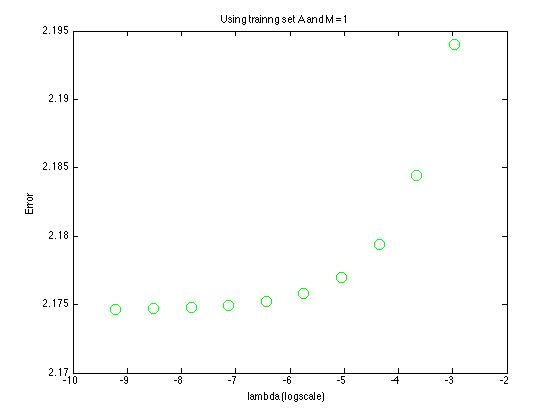
\includegraphics[width=\linewidth]{figures/p4_LASSO_regressA_m=1}
\endminipage\hfill
\minipage{0.25\textwidth}
  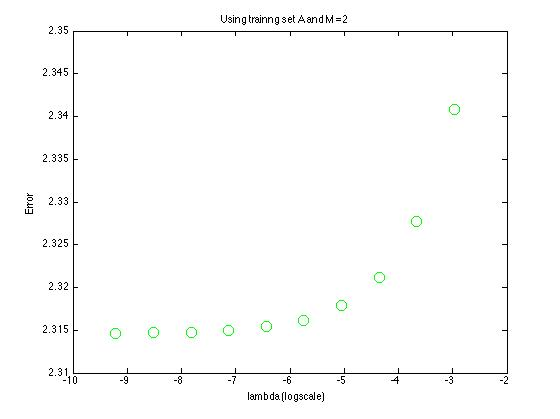
\includegraphics[width=\linewidth]{figures/p4_LASSO_regressA_m=2}
\endminipage\hfill
\minipage{0.25\textwidth}                                                                                 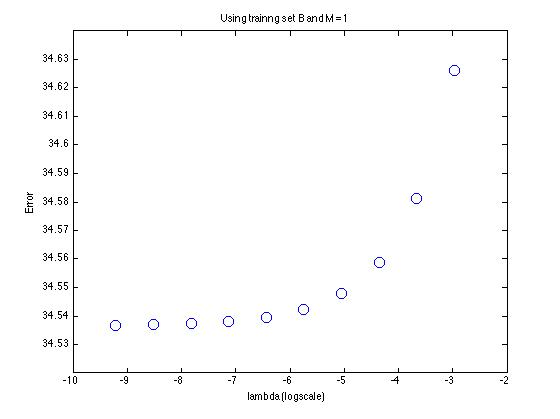
\includegraphics[width=\linewidth]{figures/p4_LASSO_regressB_m=1}
\endminipage\hfill
\minipage{0.25\textwidth}
  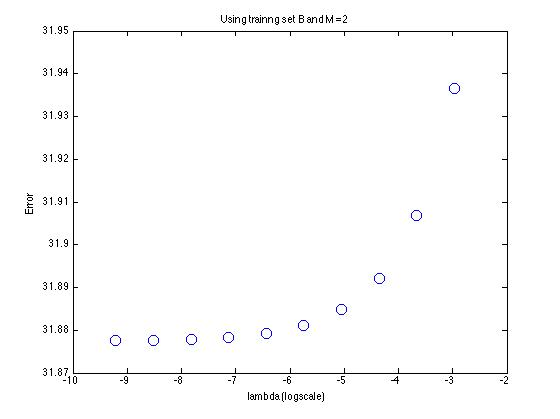
\includegraphics[width=\linewidth]{figures/p4_LASSO_regressB_m=2}
\endminipage\hfill
\caption{LASSO validation error using set A, M = 1,2 and B, M = 1,2}\label{fig:p4_LASSO}
\end{figure}


The error rate for LASSO increases quickly for M = 2 and M = 3.

{\bfseries 4.3 Part3}

We want to use the least absolute deviations
when we believe that there are outliers in your training data. As we can see, model trained using LAD
has much lower error rate compare to LASSO and SSE on training set B. When we are confident about the quality of the data (very few or no outliers), then using a squared error loss function would be more accurate in training the model. LASSO uses L1 norm for regularization to make the weight factors more sparse. 
%TODO: add more content to the explanation
I tried using larger Ms and noticed more weights are driven to 0 when using Lasso. 


\end{document}


